% !TEX program = pdflatex
% Generated by md2tex.py from interim-nov3.md. Edit the Markdown source and rebuild, not this file.
\documentclass[11pt,letterpaper]{article}

\usepackage[utf8]{inputenc}
\usepackage[T1]{fontenc}
\usepackage{newtxtext}
\usepackage{newtxmath}
\usepackage[letterpaper,margin=1in,headheight=14pt,headsep=0.25in,footskip=0.5in]{geometry}
\usepackage{graphicx}
\usepackage{array}
\usepackage{booktabs}
\usepackage{xcolor}
\usepackage{caption}
\usepackage{enumitem}
\usepackage{fancyhdr}
\usepackage{titlesec}
\usepackage{microtype}
\usepackage[hidelinks]{hyperref}

\hypersetup{pdftitle={ECSE 557: Interim Report}}

% ---------------------------------------------------------------- colours (as in the Word version)
\definecolor{boinggreen}{RGB}{0,176,80}
\definecolor{phyellow}{RGB}{255,255,0}
\definecolor{boxfill}{HTML}{F2F8EE}
\definecolor{boxline}{HTML}{A9D18E}

% ---------------------------------------------------------------- paragraphs
\setlength{\parindent}{0pt}
\setlength{\parskip}{5pt plus 1pt minus 1pt}
\setlength{\emergencystretch}{1.5em}
\widowpenalty=3000
\clubpenalty=3000

% ---------------------------------------------------------------- headings (they carry their own numbers)
\setcounter{secnumdepth}{0}
\titleformat{\section}{\normalfont\fontsize{14}{17}\selectfont\bfseries\color{boinggreen}\raggedright}{}{0pt}{}
\titlespacing*{\section}{0pt}{12pt plus 3pt minus 2pt}{2pt}
\titleformat{\subsection}{\normalfont\fontsize{11.5}{14}\selectfont\bfseries\raggedright}{}{0pt}{}
\titlespacing*{\subsection}{0pt}{9pt plus 2pt minus 1pt}{1pt}
\titleformat{\subsubsection}{\normalfont\normalsize\bfseries\itshape\raggedright}{}{0pt}{}
\titlespacing*{\subsubsection}{0pt}{7pt plus 2pt minus 1pt}{0pt}

% ---------------------------------------------------------------- lists, captions, tables
\setlist{leftmargin=0.3in,itemsep=2pt,parsep=0pt,topsep=2pt,partopsep=0pt}
\setlist[enumerate]{label=\arabic*.}
\captionsetup{font=small,labelfont=bf,justification=raggedright,singlelinecheck=false}
\captionsetup[table]{position=top,skip=4pt}
\captionsetup[figure]{position=bottom,skip=4pt}
\setlength{\tabcolsep}{4pt}
\newcommand{\rowrule}{\midrule[0.2pt]}
\setlength{\textfloatsep}{12pt plus 2pt minus 2pt}
\setlength{\floatsep}{10pt plus 2pt minus 2pt}
\setlength{\intextsep}{10pt plus 2pt minus 2pt}
\renewcommand{\topfraction}{0.9}
\renewcommand{\bottomfraction}{0.8}
\renewcommand{\textfraction}{0.07}
\renewcommand{\floatpagefraction}{0.75}

% ---------------------------------------------------------------- placeholders: [text] highlighted yellow
% Each word is a yellow box; the gaps are yellow leaders that can still break across lines.
\DeclareRobustCommand{\phword}[1]{{\setlength{\fboxsep}{0pt}\colorbox{phyellow}{\strut #1}}}
\DeclareRobustCommand{\phgap}{{\color{phyellow}\leaders\hrule height\ht\strutbox depth\dp\strutbox\hskip 0.3em plus 0.15em minus 0.08em}}

% ---------------------------------------------------------------- a light box (<!-- box -->)
\newsavebox{\reportboxbin}
\newlength{\reportboxsep}
\setlength{\reportboxsep}{6pt}
\newenvironment{reportbox}
  {\par\smallskip\noindent\begin{lrbox}{\reportboxbin}%
   \begin{minipage}{\dimexpr\linewidth-2\reportboxsep-1.2pt\relax}%
   \small\setlength{\parskip}{4pt plus 1pt}\setlength{\parindent}{0pt}}
  {\end{minipage}\end{lrbox}%
   {\setlength{\fboxsep}{\reportboxsep}\setlength{\fboxrule}{0.6pt}%
    \fcolorbox{boxline}{boxfill}{\usebox{\reportboxbin}}}\par\medskip}

% ---------------------------------------------------------------- references: hanging indent
\newenvironment{references}
  {\par\small\raggedright\setlength{\parskip}{3pt plus 1pt}\setlength{\parindent}{0pt}}
  {\par}
\newcommand{\refentry}{\par\noindent\hangindent=0.3in\hangafter=1\relax}

% ---------------------------------------------------------------- header (the frog) and page numbers
\newcommand{\headerfrog}{\makebox[0pt][l]{\hspace*{-0.19in}\raisebox{-0.33in}[0pt][0pt]{%
  
\includegraphics[width=1in]{figures/boing-frog.png}}}}
\newcommand{\coverlogo}{\makebox[0pt][l]{\hspace*{-0.44in}\raisebox{-0.355in}[0pt][0pt]{%
  
\includegraphics[width=2.49in]{figures/mcgill-logo.png}}}}
\pagestyle{fancy}
\fancyhf{}
\renewcommand{\headrulewidth}{0pt}
\renewcommand{\footrulewidth}{0pt}
\fancyhead[R]{\headerfrog}
\fancyfoot[C]{\fontsize{9}{11}\selectfont\thepage}
\fancypagestyle{cover}{%
  \fancyhf{}%
  \renewcommand{\headrulewidth}{0pt}%
  \renewcommand{\footrulewidth}{0pt}%
  \fancyhead[L]{\coverlogo}%
  \fancyhead[R]{\headerfrog}}

\begin{document}

% ================================================================ cover page (as in Repport.docx)
\thispagestyle{cover}
\vspace*{2.95in}
{\centering\fontsize{22}{27}\selectfont\bfseries ECSE 557: Intro to Ethics of Intelligent Systems\par}
\vspace{6pt}
{\centering\fontsize{16}{19}\selectfont\bfseries FINAL PROJECT\par}
\vspace{4pt}
{\centering\fontsize{16}{19}\selectfont\bfseries\underline{Interim Report}\par}
\vfill
{\fontsize{14}{17}\selectfont Professor: Ajung Moon\par}
\vspace{4pt}
{\fontsize{14}{17}\selectfont Students: Amine Houari and \phword{[Teammate's}\phgap{}\phword{full}\phgap{}\phword{name]}\enskip$\cdot$\enskip Group 14\par}
\vspace{28pt}
{\centering\fontsize{14}{17}\selectfont November 3, 2026\par}
\vspace*{0.05in}
\clearpage

\section{AI-use pre-amble}

\begin{reportbox}
\textbf{System.} Claude (Anthropic), in Claude Code, October 11 to November 2, 2026; this version was drafted
with Claude Opus 5.5
\phword{[add}\phgap{}\phword{the}\phgap{}\phword{model}\phgap{}\phword{versions}\phgap{}\phword{of}\phgap{}\phword{earlier}\phgap{}\phword{sessions]}.

\textbf{Tasks, known limits and corrections.}

\begin{enumerate}
\item \textbf{Plan and rules.} Proposed our plan, the report outline and a first list of rules.
\textit{Limits:} its judgement, not our stakeholders'. \textit{Corrections:} the rules were revised to eleven
and the coach cut to a design (Section 4).
\item \textbf{References and laws.} Drafted the introduction and references, and checked the DOIs, laws and
Montréal numbers against official sources. \textit{Limits:} it can misquote sources; some official pages could
not be read automatically. \textit{Corrections:} the check corrected three Montréal numbers and showed that
the DSA does not bind BOING (Section 2.2).
\item \textbf{Code and results.} Wrote the notebooks: simulator, methods, re-ranker, privacy and fake-account
experiments, rule checker and test cases. \textit{Limits:} code can run without doing what its text says; the
simulator's rates are arbitrary. \textit{Corrections:} automatic checks and clean re-runs; two reviews in
separate Claude sessions, which can share its blind spots, found real problems, since fixed and re-run
(Section 4).
\item \textbf{Figures.} Drew Figures 1--3 and the charts. \textit{Limits:} a diagram can look tidier than the
code. \textit{Corrections:} Figure 3 is marked illustrative; results are quoted from saved files.
\item \textbf{Report text.} Drafted this report, including this pre-amble. \textit{Limits:} the wording is its
own; it can present a hypothesis as a finding. \textit{Corrections:} every result was copied from a saved file
named in the text.
\item \textbf{Build tools.} Wrote the scripts that build this report in Word and PDF. \textit{Limits:}
conversions can fail silently. \textit{Corrections:} every PDF page was inspected.
\end{enumerate}

\phword{[What}\phgap{}\phword{we}\phgap{}\phword{checked}\phgap{}\phword{or}\phgap{}\phword{changed}\phgap{}\phword{ourselves:}\phgap{}\phword{e.g.}\phgap{}\phword{re-ran}\phgap{}\phword{the}\phgap{}\phword{notebooks,}\phgap{}\phword{checked}\phgap{}\phword{the}\phgap{}\phword{sources,}\phgap{}\phword{rewrote}\phgap{}\phword{sections}\phgap{}\phword{(say}\phgap{}\phword{which).]}

\textbf{Reflection.} Using Claude let us build and test far more than we could have alone in this time, but it
also changed what our work was. We spent less time writing code and more time checking whether we understood
and agreed with what it produced. For example, while reading the report I realised it had narrowed our project
to group suggestions, leaving out the friend and feed suggestions in our plan, without asking me. I also had
to ask it to explain ideas like fair re-ranking and the hidden tastes model in simple terms before I could
defend them. The biggest lesson for a course on responsible AI is that clean, confident output can still be
wrong, as when a review showed that our first privacy setting did not hold up on new tests, so we now treat
its work as a draft to question rather than an answer to trust.

\end{reportbox}

\section{1. Design Context}

Recommender systems shape much of what people see online. Most of them are tuned for engagement, mainly
because engagement is easy to measure, even though it is only a rough stand-in for what people actually value
(Kleinberg et al., 2022). Engagement-driven systems have been linked to filter bubbles (Pariser, 2011) and to
popularity bias, where a few items take most of the attention (Abdollahpouri et al., 2017). They can also
create feedback loops that make behaviour more homogeneous (Chaney et al., 2018), and the profiling behind
them intrudes on privacy and autonomy (Milano et al., 2020). Platforms usually add these systems once they are
already large. A new platform has the chance to decide what its recommender is for before building it.

\textbf{BOING.} BOING is a free social network where a member's identity is a character rather than a
photograph. Members join groups around personal goals such as languages, coding or exam preparation, plan
their week with an AI coach and play games. They sign up with a username and either an email address or a
crypto wallet (email sign-up is being added). No real name is required, and the audience includes teenagers.
BOING already enforces privacy and safety rules (private profiles, blocking, reports, human moderators), but
it has no recommender. Its Discover page ranks groups by member count, so large groups keep growing while new
ones stay invisible.

\textbf{What we design.} We start with a recommender that suggests groups to join, which is built and tested.
For the final report, we are extending the design to suggesting people and to a personalised feed of posts,
guided by the same values and rules, and going as deep as time allows. Its objective is to help members find
groups that suit them while keeping new groups visible, protecting privacy by default and resisting fake
accounts. This objective and its constraints come from what stakeholders value, not from engagement. It serves
BOING's members, including newcomers and teenagers, but it also affects the groups it ranks and the members
whose activity feeds it.

\textbf{Deployment assumptions.} Our design rests on seven assumptions:

\begin{enumerate}
\item The network is small and young, so popularity bias would lock in early winners.
\item Sign-up needs no real identity. Wallets and ordinary email addresses are cheap to create, so fake
(``Sybil'') accounts are too, although a verified campus address would make them harder.
\item Members will give a birth year at sign-up, kept private and used only for safety. It is not verified, so
suggesting people must be conservative.
\item BOING's mission is helping people reach their goals, not keeping them on the site, so success means a
short list of useful suggestions rather than clicks.
\item BOING is subject to Quebec's private-sector privacy act as amended by Law 25 (S.Q. 2021, c. 25).
\item We use no real-user data. We evaluate on a synthetic community and a local copy of BOING with fake
members.
\item BOING launches first at McGill, as a campus space inside the wider BOING world, then at other campuses.
BOING is independent of the university, and we do not test a campus filter here.
\end{enumerate}

\textbf{Approach.} Following value sensitive design (Friedman \& Hendry, 2019), we identify the stakeholders,
their values and the tensions between them. We then use the Montréal Declaration (Université de Montréal,
2018) to turn these values into eleven testable design rules. Some are hard limits that are never traded:
personalisation is opt-in, private data is never used, and money cannot buy visibility. Others are dials that
we tune through experiments, namely fair exposure for new groups, diversity, resistance to fake accounts and
differential privacy. We test the design against BOING's current ranking on a synthetic community of 2,000
users and 150 groups, and measure what each value costs in accuracy. Section 2 presents the design, Section 3
covers the evaluation and our first results, and Section 4 describes our progress and the plan for the final
report.

\section{2. Design}

\subsection{2.1 Stakeholders and values}

Following value sensitive design, we list everyone the recommender affects, including indirect stakeholders
who never see it, such as members whose memberships shape other people's suggestions (Table 1). Because we
have no real users, the values come from BOING's policies (no paid advantages, private spaces stay private,
safety tools for teenagers), published work on recommender harms and our own judgement. Not having a study
with real users is a limitation.

\begin{table}[!htbp]
\centering
\caption*{\textbf{Table 1.} Stakeholders of the recommender and the values at stake.}
\scriptsize
\begin{tabular}{
  >{\raggedright\arraybackslash}p{\dimexpr 0.3462\linewidth-2\tabcolsep\relax}
  >{\raggedright\arraybackslash}p{\dimexpr 0.1769\linewidth-2\tabcolsep\relax}
  >{\raggedright\arraybackslash}p{\dimexpr 0.4769\linewidth-2\tabcolsep\relax}
}
\toprule
\textbf{Stakeholder} & \textbf{Type} & \textbf{Values at stake} \\
\midrule
Members looking for groups & Direct & Relevance, autonomy (control), privacy, well-being \\
\rowrule
New members; new and small groups & Direct & A fair chance to be seen (equity), belonging \\
\rowrule
Teenage members & Direct, vulnerable & Safety, privacy, not being pushed towards strangers \\
\rowrule
Group owners & Direct & Visibility; protection from manipulation by rivals \\
\rowrule
Members whose data feeds others' suggestions & Indirect & Privacy: not being inferred or exposed through ``people like you'' \\
\rowrule
Moderators & Indirect & Not amplifying hidden or reported content; a manageable workload \\
\rowrule
Parents and schools & Indirect & Safety, healthy use \\
\rowrule
The platform operator & Indirect & Trust, growth, legal compliance \\
\bottomrule
\end{tabular}
\end{table}

These values pull against each other in five places (Table 2). We call a conflict a \textit{tension} when a
careful design can mostly resolve it, and a \textit{trade-off} when gaining one value costs another, so that
an experiment has to measure the price. Rules can conflict as well. Counting only established accounts (R9)
protects group owners from fake accounts, but it also delays the weight of a new member's joins, and
experiments E4 and E5 measure both effects.

\begin{table}[!htbp]
\centering
\caption*{\textbf{Table 2.} Value tensions, how the design serves both sides, and the experiment (Table 5)
that settles each one.}
\scriptsize
\begin{tabular}{
  >{\raggedright\arraybackslash}p{\dimexpr 0.2385\linewidth-2\tabcolsep\relax}
  >{\raggedright\arraybackslash}p{\dimexpr 0.1462\linewidth-2\tabcolsep\relax}
  >{\raggedright\arraybackslash}p{\dimexpr 0.4000\linewidth-2\tabcolsep\relax}
  >{\raggedright\arraybackslash}p{\dimexpr 0.2154\linewidth-2\tabcolsep\relax}
}
\toprule
\textbf{Tension} & \textbf{Kind} & \textbf{How the design serves both} & \textbf{Settled by} \\
\midrule
Relevance vs fair exposure & Partly a trade-off & Reserve 1--2 of the 5 slots for the most relevant new or small groups, not random ones & E2: accuracy vs newcomer share \\
\rowrule
Personalisation vs privacy & Tension & Opt-in (R1), an allow-list of data (R2), noisy statistics (R10) & E3: accuracy vs $\varepsilon$ \\
\rowrule
Transparency vs manipulation & Tension & Explain the kind of reason, not the weights; R9 limits gaming & E4, with reasons shown \\
\rowrule
Discovery vs safety & Tension & People are suggested only through a shared group or friend (R8) & E6: zero violations \\
\rowrule
Engagement vs well-being & Tension & Five suggestions, no endless list, no notifications (R11) & List length; topic match \\
\bottomrule
\end{tabular}
\end{table}

\subsection{2.2 From values to design rules}

We turn values into rules with a values hierarchy (van de Poel, 2013). Each value is specified as norms that
say what it demands on BOING, and each norm becomes a requirement we can test (Figure 1). Every rule is traced
to the principles and items of the Montréal Declaration (Université de Montréal, 2018). For R1, we rely on
sections 9.1 and 8.1 of Quebec's private-sector act (CQLR c P-39.1), both added by Law 25. They require ``the
highest level of confidentiality by default, without any intervention by the person concerned'', and they
require telling people first that a technology able to profile them is used and how to activate it. Profiling
includes assessing ``personal preferences, interests or behaviour'', which is what a taste model does. We read
these sections together as support for R1, so profiling stays off until the member switches it on. This is our
own reading, and we have not checked the regulator's guidance. The EU Digital Services Act (2022) does not
bind BOING, since Article 19 exempts small enterprises from Article 27 and Article 38 covers only very large
platforms. We still follow it voluntarily. R6 and R7 aim at Article 27, and R1 goes further than Article 38 by
making the option without profiling the default.

We take a pluralist stance. Seven rules are hard limits that are never traded and are tested to zero
violations. These cover the safety filters, the privacy of private spaces and the ban on paying for reach. The
other four are dials whose settings come from the experiments, and the Discussion of the final report will
defend them (Table 3). This follows the Declaration itself, whose principles are not ranked but limit one
another: ``the limits of one principle's application are defined by another principle's field of application''
(p. 5).

\textbf{Social and policy implications.} Socially, the design gives new groups a fair chance of being seen,
and it limits who can be reached through suggestions. On policy, it treats privacy by default as a requirement
under Quebec law, and it follows the Digital Services Act as a voluntary benchmark.

\begin{figure}[!htbp]
\centering
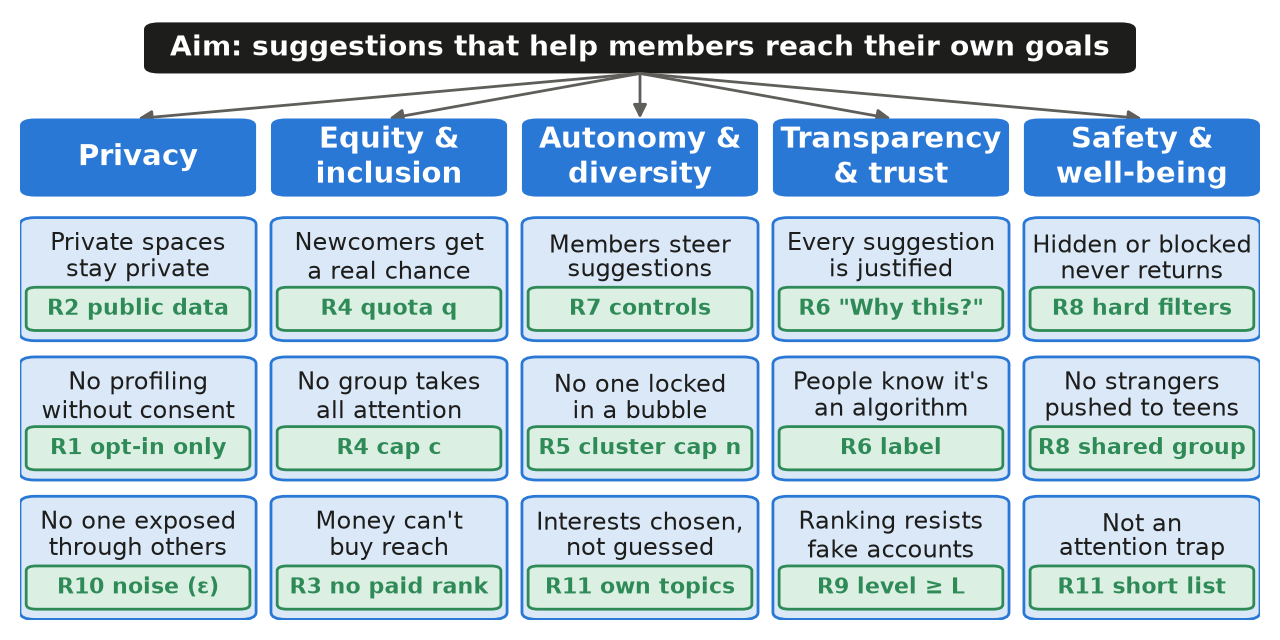
\includegraphics[width=4.7in,height=0.75\textheight,keepaspectratio]{figures/values-hierarchy.png}
\caption*{\textbf{Figure 1.} Values hierarchy of the recommender (after van de Poel, 2013). Each value (top)
is specified as norms, and each norm becomes a testable design rule (Table 3).}
\end{figure}

\begin{table}[!htbp]
\centering
\caption*{\textbf{Table 3.} The design rules. Hard rules are never traded; dial rules are tuned by the
experiments. Montréal numbers are principle.item of the Declaration (Université de Montréal, 2018); ``Law 25''
means sections 8.1 and 9.1 of Quebec's private-sector act.}
\scriptsize
\begin{tabular}{
  >{\raggedright\arraybackslash}p{\dimexpr 0.0846\linewidth-2\tabcolsep\relax}
  >{\raggedright\arraybackslash}p{\dimexpr 0.4538\linewidth-2\tabcolsep\relax}
  >{\raggedright\arraybackslash}p{\dimexpr 0.1415\linewidth-2\tabcolsep\relax}
  >{\raggedright\arraybackslash}p{\dimexpr 0.1200\linewidth-2\tabcolsep\relax}
  >{\raggedright\arraybackslash}p{\dimexpr 0.2000\linewidth-2\tabcolsep\relax}
}
\toprule
\textbf{Rule} & \textbf{What the recommender must do} & \textbf{Values} & \textbf{Montréal} & \textbf{Passes when} \\
\midrule
\textbf{R1}\mbox{}\newline Hard & Opt-in: personalised suggestions are off until a member turns them on. With them off, the page still lists new, active and curated groups. & Privacy, autonomy & 3.4, 3.6; Law 25 & New accounts start off; the off list is never empty \\
\rowrule
\textbf{R2}\mbox{}\newline Hard & Allow-list: only public, on-platform signals (memberships, likes, friendships, public posts, group descriptions, topics a member picked). Never messages, planner, coach chats, purchases, wallets, email addresses or birth years. & Privacy & 3.1, 3.2, 8.4 & Changing a member's private data changes nothing in their suggestions \\
\rowrule
\textbf{R3}\mbox{}\newline Hard & No paying for reach: tokens, purchases and ads never change the ranking; ads stay a separate, labelled slot. & Equity, trust & 6.2 & A group's spending does not move its rank \\
\rowrule
\textbf{R4}\mbox{}\newline Dial q, c & Fair exposure: at least q\% of all slots go to new (30 days or less) or small (under 10 members) groups; no group takes more than c\% of all slots. & Equity, inclusion & 6.2, 6.3, 7.1 & Newcomer share $\geq$ q; largest share $\leq$ c; Gini reported \\
\rowrule
\textbf{R5}\mbox{}\newline Dial n, $\lambda$ & Diversity: at most n of the 5 suggestions share a topic; similar groups are spread out. & Autonomy, diversity & 7.1, 7.4 & No list breaks n \\
\rowrule
\textbf{R6}\mbox{}\newline Hard & Honest reasons: each suggestion shows its main true reason from a fixed template and is labelled as made by an algorithm. A friend is named only if their profile is public. & Transparency, privacy & 5.2, 5.7, 5.8 & Explanation fidelity is 100\% \\
\rowrule
\textbf{R7}\mbox{}\newline Hard & Members steer: ``Not interested'', hide a topic, reset, see what is used. The system only suggests; it never joins or messages anyone for a member. & Autonomy & 2.1, 3.4, 3.6, 9.2 & Hidden items never return; reset clears everything \\
\rowrule
\textbf{R8}\mbox{}\newline Hard & Safety filters: never suggest blocked, suspended or private accounts, or anything hidden by moderators or reports. People only through a shared group or a friend of a friend. & Safety & 1.5, 3.1, 4.1, 8.3 & Zero violations on the test cases \\
\rowrule
\textbf{R9}\mbox{}\newline Dial L, w & Fake-account resistance: only established accounts (level L or more) count, each once; joins by accounts younger than 30 days count less (weight w). & Trust, fairness & 8.3, 6.2 & Places a target group climbs per fake account \\
\rowrule
\textbf{R10}\mbox{}\newline Dial $\varepsilon$, m & Differential privacy: statistics about other members get calibrated noise, and each member counts for at most m groups. & Privacy & 3.5, 8.4 & Accuracy at each $\varepsilon$ (privacy--utility curve) \\
\rowrule
\textbf{R11}\mbox{}\newline Hard & Well-being: five suggestions, no endless scroll, no notifications. Topic matching uses only topics members chose, never topics inferred from their activity. & Well-being, autonomy & 1.5, 2.6, 3.3 & Lists have 5 items; no inferred topics used \\
\bottomrule
\end{tabular}
\end{table}

The experiments sweep each dial: q $\in$ \{0, 20, 40, 60\}\% and c $\in$ \{5\%, 10\%, no cap\} for R4; n $\in$
\{2, 3, 5\} and the variety weight $\lambda \in$ \{0.5, 0.7, 0.8, 0.9, 1\} for R5; L $\in$ \{1, 3, 5\} and w
$\in$ \{0, 1\} for R9; and $\varepsilon \in$ \{0.1, 0.5, 1, 2, 5, $\infty$\} with m $\in$ \{3, 5, 8\} for R10.
Three choices are fixed rather than tuned: five suggestions, ``new'' means created in the last 30 days, and
``small'' means fewer than 10 members.

\subsection{2.3 The system}

Figure 2 shows how a suggestion is made. Once a night, BOING reads only the allowed data (R2) and computes
every statistic about other members in one place, so the rules about whose data counts (R8--R10) reach every
score at once. When a member who has switched personalisation on opens the Groups page, the candidate groups
are scored, filtered (R7, R8) and re-ranked (R4, R5), and five suggestions are shown with their reasons (R6).
Only the scoring step is learned. Every ethical guarantee sits in fixed, testable steps around it, so changing
the model cannot break a hard rule. By default personalisation is off, so no profile is used, and the same
filtering and re-ranking apply to new and active groups (R1). Table 4 shows how our prototype builds each
step. A rule checker counts every hard-rule violation, and we plant faults on purpose to show that each check
can fire. The chosen design will run on a local test copy of BOING with fake members only.

\begin{figure}[!htbp]
\centering
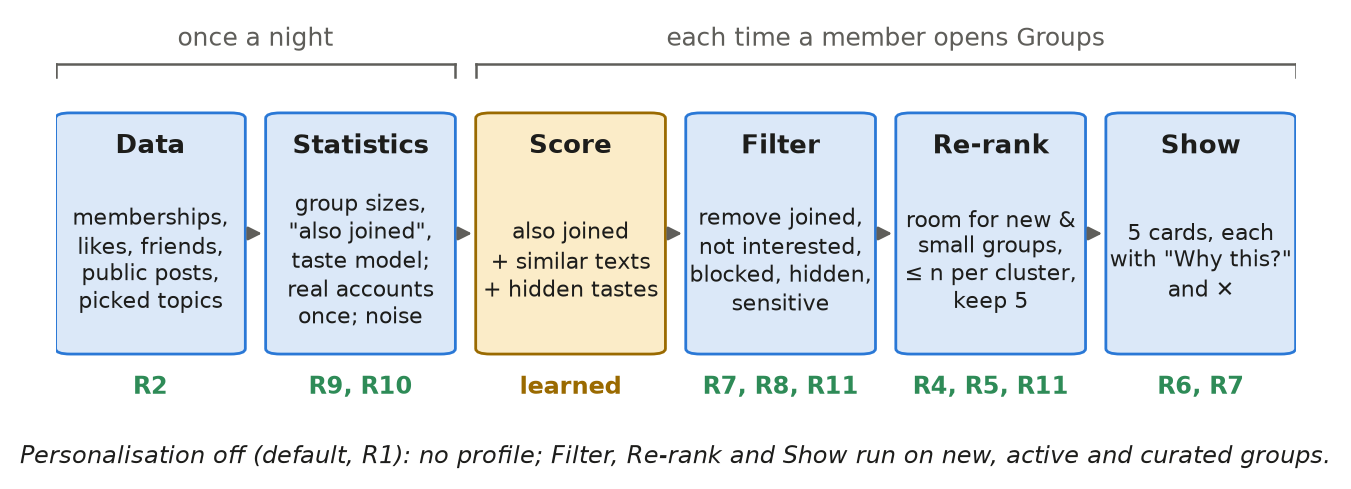
\includegraphics[width=5.2in,height=0.75\textheight,keepaspectratio]{figures/pipeline.png}
\caption*{\textbf{Figure 2.} How a suggestion is made, and the rules each step enforces. Only the amber step
is learned; it also counts public friends who are members, which the diagram does not show (Section 2.4).}
\end{figure}

\begin{table}[!htbp]
\centering
\caption*{\textbf{Table 4.} How the prototype enforces the rules at each step of Figure 2, and where each step
stands on November 1.}
\scriptsize
\begin{tabular}{
  >{\raggedright\arraybackslash}p{\dimexpr 0.1692\linewidth-2\tabcolsep\relax}
  >{\raggedright\arraybackslash}p{\dimexpr 0.6615\linewidth-2\tabcolsep\relax}
  >{\raggedright\arraybackslash}p{\dimexpr 0.1692\linewidth-2\tabcolsep\relax}
}
\toprule
\textbf{Step (rules)} & \textbf{How the prototype does it} & \textbf{Status} \\
\midrule
Data (R2, R3) & Only the allowed tables reach the recommender. A check alters private data and paid budgets and confirms that no list changes. & Built \\
\rowrule
Statistics (R8--R10) & One function makes every count about other members: no suspended accounts; only level L or more, once each, young ones with weight w; at most m groups per member; Laplace noise for $\varepsilon$. & Built; re-checked \\
\rowrule
Filter (R7, R8) & Open, unhidden Discover groups the member has not joined or dismissed; a friend counts only with a public profile and no block. & Built \\
\rowrule
Re-rank (R4, R5, R11) & Greedy, slot by slot: quota q, cap c, at most n groups per topic cluster, variety $\lambda$; five slots. & Built; dials fixed \\
\rowrule
Show (R6, R7) & One template reason each: the part that adds most to the score, or ``a fair chance'' for a quota slot. ``Not interested'' is permanent. & Built; more controls planned \\
\rowrule
Off, the default (R1) & No profile: recent activity and newness, then the same filter and re-ranking. & Built \\
\bottomrule
\end{tabular}
\end{table}

\subsection{2.4 The algorithms}

We built the scoring step up from the simplest method, so that each addition has to beat the simpler ones.
Learned methods see only the training data, and every setting is chosen on a validation split of it, never on
the test set (Section 3.1). Besides popularity, our baseline, we compare:

\begin{itemize}
\item \textit{``Also joined''}, item-to-item collaborative filtering (Sarwar et al., 2001): a group scores by
its member overlap (Jaccard) with each of the member's groups, which gives reasons such as ``4 members of X
are in it''.
\item \textit{Similar descriptions}: the TF-IDF similarity of a group's description to those of the member's
groups. It needs no members, so it reaches new groups.
\item \textit{Hidden tastes}, our AI model: a truncated SVD of the member $\times$ group matrix (Koren et al.,
2009) with 10 tastes, chosen on the validation split; on 0/1 join data with no missing entries, plain SVD is a
reasonable first model. Its tastes line up with the hidden topics it never sees. Because it profiles members,
it is opt-in (R1).
\item \textit{Friends}: how many of the member's friends with a public profile are in the group.
\item The \textit{hybrid} rescales each score to 0--1 over the member's candidates and mixes them with weights
chosen on the validation split among 286 mixes: 0.4 ``also joined'', 0.1 descriptions, 0.3 friends and 0.2
hidden tastes. The best mixes differ by thousandths; the final design re-chooses them with the privacy noise
on.
\item The \textit{fair re-ranker} fills each list one slot at a time, trading relevance against similarity to
the groups already picked ($\lambda$; Carbonell \& Goldstein, 1998), with quota q, cap c and at most n groups
per topic cluster (clusters of the descriptions, since the hidden topics may not be read).
\end{itemize}

The re-ranker applies the idea of fairness of exposure: a ranking shares out attention, and that share can be
held to a standard (Singh \& Joachims, 2018). Like them, we keep fairness to groups (R4) separate from variety
for the member (R5). For R10, each member counts for at most m groups, and Laplace noise calibrated to
$\varepsilon$ is added to the group sizes and pair counts (Dwork \& Roth, 2014). ``Also joined'' and the taste
model both come from these counts, so one noisy release protects both (McSherry \& Mironov, 2009). Public
signals are not covered, and the final report will state the guarantee's exact scope. R9 is our defence
against Sybil attacks (Douceur, 2002), which push little-known items most easily (Lam \& Riedl, 2004).
Tournesol takes a similar approach by counting only trusted accounts (Hoang et al., 2021). Each reason is
meant to support transparency and scrutability (Tintarev \& Masthoff, 2007), not persuasion.

\subsection{2.5 The interface}

Figure 3 sketches the new Groups page. With personalisation off, every member sees the same list of new and
active groups. With it on, the five suggestions are labelled as made by an algorithm, and each shows its
reason and can be dismissed (R6, R7). We will build it on the local test copy of BOING (Section 4).

\begin{figure}[!htbp]
\centering
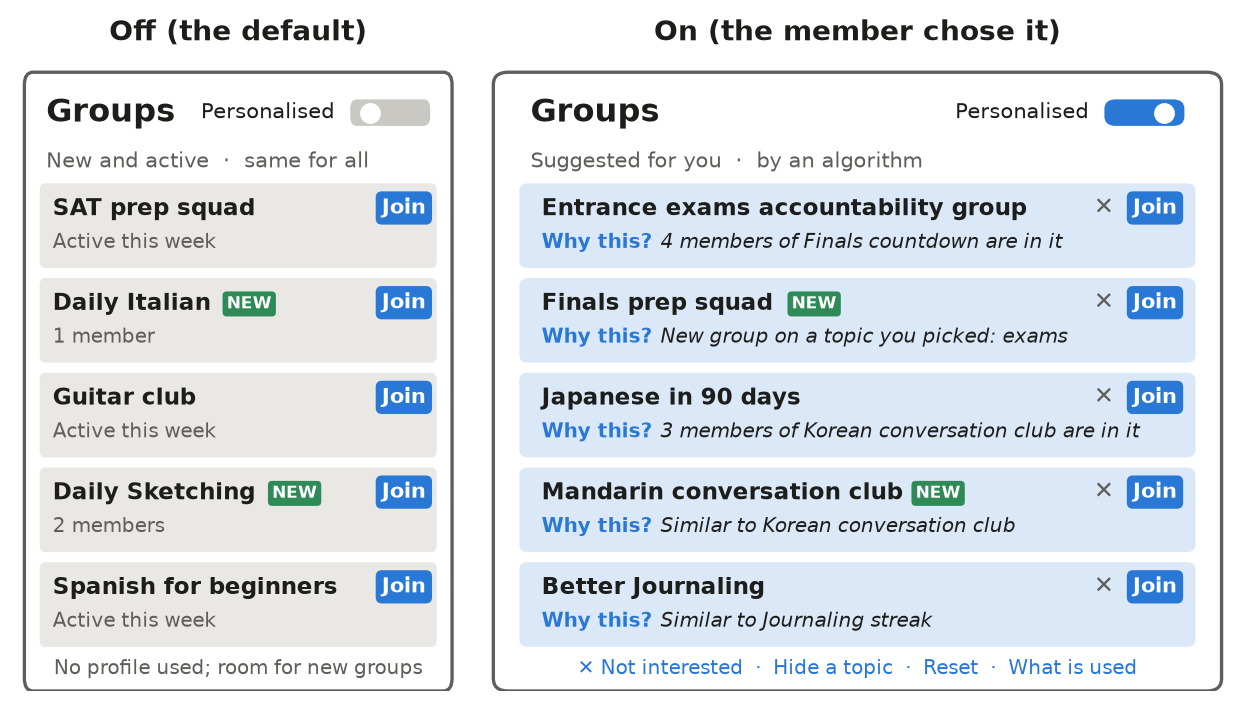
\includegraphics[width=3.5in,height=0.75\textheight,keepaspectratio]{figures/groups-screen-sketch-interim.png}
\caption*{\textbf{Figure 3.} Sketch of the new Groups page for user 1 of the synthetic community (Section
3.2). Left: the default, with no profiling. Right: after the member switches personalisation on. The group
names come from the synthetic data; the suggestions are illustrative, not the output of a method.}
\end{figure}

\section{3. Evaluation Plan and First Results}

\subsection{3.1 A synthetic community}

We evaluate on synthetic data only, so no member's data is collected. A simulator generates 2,000 users and
150 groups across 10 topics, such as exam preparation, languages and coding. Each user has hidden interests in
1 to 3 topics and each group a hidden topic. Joins happen in time order. In 88\% of cases they go to a user's
favourite topics and otherwise they are random, and either way bigger groups are more likely to be picked.
This ``rich get richer'' rule reproduces the long tail of real platforms. The ten largest groups hold 35\% of
all memberships, while 64 groups have fewer than 10 members. Fifteen percent of users and 20\% of groups are
new. Blocks, suspended accounts and three groups hidden by moderators let us test the safety rules. The hidden
interests and topics act as the answer key, and only the scoring code reads them. These rates are our
assumptions about behaviour, not measurements, and a fixed random seed makes every result reproducible. Table
5 lists the experiments we run on it, and where each stands.

\begin{table}[!htbp]
\centering
\caption*{\textbf{Table 5.} The experiments, and where each stands on November 1.}
\scriptsize
\begin{tabular}{
  >{\raggedright\arraybackslash}p{\dimexpr 0.0538\linewidth-2\tabcolsep\relax}
  >{\raggedright\arraybackslash}p{\dimexpr 0.4077\linewidth-2\tabcolsep\relax}
  >{\raggedright\arraybackslash}p{\dimexpr 0.2846\linewidth-2\tabcolsep\relax}
  >{\raggedright\arraybackslash}p{\dimexpr 0.1154\linewidth-2\tabcolsep\relax}
  >{\raggedright\arraybackslash}p{\dimexpr 0.1385\linewidth-2\tabcolsep\relax}
}
\toprule
\textbf{\#} & \textbf{Question} & \textbf{What we measure} & \textbf{Rules} & \textbf{Status} \\
\midrule
E1 & Which scoring method works best, with and without fair re-ranking? & Relevance, exposure, diversity & All & Done (Section 3.3) \\
\rowrule
E2 & What do fair exposure and variety cost (q, c, n, $\lambda$)? & NDCG@5 against newcomer share & R4, R5 & Done; values in the final report \\
\rowrule
E3 & What does privacy cost ($\varepsilon$, m)? Opted-in members only against everyone & NDCG@5 against $\varepsilon$ & R10 & Re-checked; values in the final report \\
\rowrule
E4 & Can 0.5--10\% fake accounts of four kinds push a small new group up? & Lists showing the target; places gained per fake & R9 & Re-checked; values in the final report \\
\rowrule
E5 & Do new members and new groups get a fair deal? & NDCG@5 by groups joined; new groups' exposure & R4, R9 & Done; values in the final report \\
\rowrule
E6 & Do the hard rules hold? & Violations (target 0); faithful reasons (100\%); planted faults caught & R1--R3, R6--R8, R11 & Done; values in the final report \\
\bottomrule
\end{tabular}
\end{table}

\textbf{Test set and metrics.} For the 1,406 users with at least three groups, we hide 20\% of their
memberships (at least one). This gives 1,531 hidden memberships for the test set and leaves 6,428 visible, and
we remove any posts or likes that would reveal a hidden membership. To choose settings, we hide 20\% of the
visible memberships again in the same way, which keeps the test set for reporting only. Each method gives each
user five suggestions. Relevance is measured with the hit rate (the share of users for whom at least one
suggestion is a hidden group), precision@5, recall@5 and NDCG@5, which gives more credit to a correct group
ranked higher (Järvelin \& Kekäläinen, 2002). Fair exposure (R4) is the share of slots that go to new or small
groups, alongside the Gini coefficient of exposure and the number of groups ever shown. Diversity (R5) is the
number of topics per list.

\subsection{3.2 First results: today's ranking}

We scored BOING's current ranking on the test set (the largest open groups not hidden by moderators, minus the
user's own groups), with five random groups per user as a floor. Ranking by size beats chance by more than a
factor of four: 22\% of users find a hidden group among their five suggestions, against 5\% with random
suggestions, and NDCG@5 is 0.131 (t4\_baseline.csv; Table 6). The cost shows in who gets seen. Because
everyone receives the same ranking, only 10 of the 129 groups on Discover were ever suggested to the 1,406
users, and none of the 53 new or small groups appeared. The newcomer share is 0\% and the Gini coefficient of
exposure is 0.953 (t5\_exposure.csv). Relevance suffers as well. User 1, who studies for exams, is offered
large groups on weightlifting, Japanese, Spanish and algorithms, and none of them is correct. This is the
popularity bias described in Section 1. It sets the relevance that every method in E1 must beat, and the 0\%
newcomer share that R4 must raise.

\subsection{3.3 First results: comparing the methods (E1)}

In Table 6, ``also joined'' (NDCG@5 0.499) and the AI model (0.475) beat today's ranking (0.131) by a wide
margin. The hybrid is the most relevant (0.541), although its 95\% range overlaps that of ``also joined''.
However, the accurate methods give new or small groups almost no slots (0.5\% to 2.7\%). They learn from
memberships, which such groups lack, so accuracy alone brings popularity bias back in a milder form. Similar
descriptions needs no members and gives them 41.6\% of its slots, but it is weak on relevance (0.159).

The fair re-ranker fixes this at a small cost. New or small groups get 20.3\% of the slots, 125 of the 129
Discover groups are shown, and the Gini coefficient of exposure falls to 0.511 (0.640 for the hybrid and 0.953
for popularity). Its NDCG@5 is 0.528, so the price of fairness is 0.0126 NDCG@5 per user on average, 2.3\% of
the hybrid's (paired 95\% range 0.008 to 0.017; e1\_price\_of\_fairness.json). The default list, with no
profile (R1), is far less relevant (0.058, against 0.025 for random) and shows only 14 groups, since every
member sees nearly the same list. This is the price of not profiling anyone. E1 makes the hybrid with fair
re-ranking our design, and E2 to E5 tune its dials and add the privacy noise and the fake-account defence.

\begin{table}[!htbp]
\centering
\caption*{\textbf{Table 6.} First comparison of the methods on the test set (E1; 1,406 users). Re-ranker: q =
20\%, c = 10\%, n = 2, $\lambda$ = 1. 95\% ranges from resampling the users; groups shown, of the 129 on
Discover. Source: results/e1\_methods.csv, e1\_methods\_ci.csv.}
\footnotesize
\begin{tabular}{
  >{\raggedright\arraybackslash}p{\dimexpr 0.3147\linewidth-2\tabcolsep\relax}
  >{\raggedleft\arraybackslash}p{\dimexpr 0.1049\linewidth-2\tabcolsep\relax}
  >{\raggedleft\arraybackslash}p{\dimexpr 0.2028\linewidth-2\tabcolsep\relax}
  >{\raggedleft\arraybackslash}p{\dimexpr 0.1538\linewidth-2\tabcolsep\relax}
  >{\raggedleft\arraybackslash}p{\dimexpr 0.1119\linewidth-2\tabcolsep\relax}
  >{\raggedleft\arraybackslash}p{\dimexpr 0.1119\linewidth-2\tabcolsep\relax}
}
\toprule
\textbf{Method} & \textbf{Hit rate} & \textbf{NDCG@5 (95\% range)} & \textbf{Slots for new or small groups} & \textbf{Gini of exposure} & \textbf{Groups shown} \\
\midrule
Random (floor) & 0.048 & 0.025 (0.019--0.033) & 41.7\% & 0.079 & 129 \\
\rowrule
Popularity (BOING today) & 0.220 & 0.131 (0.117--0.146) & 0\% & 0.953 & 10 \\
\rowrule
``Also joined'' & 0.640 & 0.499 (0.476--0.522) & 2.7\% & 0.599 & 94 \\
\rowrule
Similar descriptions & 0.263 & 0.159 (0.144--0.176) & 41.6\% & 0.502 & 125 \\
\rowrule
Hidden tastes (AI model) & 0.610 & 0.475 (0.452--0.496) & 0.5\% & 0.645 & 76 \\
\rowrule
Hybrid & 0.687 & 0.541 (0.517--0.563) & 2.0\% & 0.640 & 106 \\
\rowrule
\textbf{Hybrid + fair re-ranking} & \textbf{0.656} & \textbf{0.528 (0.504--0.551)} & \textbf{20.3\%} & \textbf{0.511} & \textbf{125} \\
\rowrule
Personalisation off (default) & 0.098 & 0.058 (0.048--0.068) & 54.7\% & 0.921 & 14 \\
\bottomrule
\end{tabular}
\end{table}

\section{4. Progress and Plan to the Final Report}

The Design is complete, the prototype implements all of Figure 2 (Table 4), and E1 to E6 have all been run.
This report gives the E1 results. Two code reviews (separate Claude sessions) found problems in how ``small''
groups are counted and in what R9 and the privacy noise cover. We fixed them and re-ran the affected results,
and the final report will give the values for E2 to E6. Test cases are ready for the port to BOING's local
test copy (Table 7).

\begin{table}[!htbp]
\centering
\caption*{\textbf{Table 7.} Progress and plan.}
\scriptsize
\begin{tabular}{
  >{\raggedright\arraybackslash}p{\dimexpr 0.1385\linewidth-2\tabcolsep\relax}
  >{\raggedright\arraybackslash}p{\dimexpr 0.7462\linewidth-2\tabcolsep\relax}
  >{\raggedright\arraybackslash}p{\dimexpr 0.1154\linewidth-2\tabcolsep\relax}
}
\toprule
\textbf{When} & \textbf{Work} & \textbf{Status} \\
\midrule
Oct 11--27 & Synthetic community, test set, baseline; stakeholders, values, design rules R1--R11, system design & Done \\
\rowrule
Oct 28 -- Nov 1 & Baseline exposure; the four scores, the hybrid and the fair re-ranker; E1; E2--E6; rule checker and test cases; two code reviews and their fixes; every dial fixed & Done \\
\rowrule
Nov 2--15 & Extend the design to suggesting people and a personalised feed of posts, with the same values and rules, as far as time allows & Starting \\
\rowrule
Nov 10--16 & Build the chosen design on BOING's local test copy and check it against the test cases; ``before'' and ``after'' screens & Planned \\
\rowrule
Nov 17--24 & Final report (Results, Discussion of the dials and stakeholders, Conclusion, a model card after Mitchell et al., 2019); slides, video; presentation Nov 24, 26 or Dec 1 & Planned \\
\bottomrule
\end{tabular}
\end{table}

\textbf{Expected results.} By the final report, the prototype will give each member who opts in five group
suggestions with their reasons, and a default list with no profile to everyone else, running on a local test
copy of BOING with fake members. We will assess it by its relevance against today's ranking (hit rate and
NDCG@5), the share of slots that go to new or small groups, the Gini coefficient of exposure, zero hard-rule
violations, and what each rule costs in accuracy. We expect it to stay well above today's ranking in relevance
while giving new or small groups about 20\% of the slots.

\textbf{Scope.} A privacy layer for BOING's AI coach was planned as a second part. The TA warned that doing
both would be a lot of work, so it becomes a design and audit in the final Discussion, with no code.
\textbf{Known limitations.} Synthetic data encode our own assumptions, so we trust the trade-offs more than
the absolute numbers. Relevance here means rejoining a hidden group, not being satisfied with it. The values
come from documents and our judgement rather than interviews. Ages are unverified, so teen protections apply
to everyone.

\section{References}

\begin{references}
\refentry Abdollahpouri, H., Burke, R., \& Mobasher, B. (2017). Controlling popularity bias in
learning-to-rank recommendation. In \textit{Proceedings of the Eleventh ACM Conference on Recommender Systems}
(pp. 42--46). Association for Computing Machinery. \url{https://doi.org/10.1145/3109859.3109912}

\refentry Act respecting the protection of personal information in the private sector, CQLR c P-39.1, ss. 8.1,
9.1 (consolidated to October 15, 2026). \url{https://www.legisquebec.gouv.qc.ca/en/document/cs/P-39.1}

\refentry An Act to modernize legislative provisions as regards the protection of personal information, S.Q.
2021, c. 25 (assented to September 22, 2021).
\url{https://www.assnat.qc.ca/en/travaux-parlementaires/projets-loi/projet-loi-64-42-1.html}

\refentry Carbonell, J., \& Goldstein, J. (1998). The use of MMR, diversity-based reranking for reordering
documents and producing summaries. In \textit{Proceedings of the 21st Annual International ACM SIGIR
Conference on Research and Development in Information Retrieval} (pp. 335--336). Association for Computing
Machinery. \url{https://doi.org/10.1145/290941.291025}

\refentry Chaney, A. J. B., Stewart, B. M., \& Engelhardt, B. E. (2018). How algorithmic confounding in
recommendation systems increases homogeneity and decreases utility. In \textit{Proceedings of the 12th ACM
Conference on Recommender Systems} (pp. 224--232). Association for Computing Machinery.
\url{https://doi.org/10.1145/3240323.3240370}

\refentry Douceur, J. R. (2002). The Sybil attack. In P. Druschel, F. Kaashoek, \& A. Rowstron (Eds.),
\textit{Peer-to-peer systems: First International Workshop, IPTPS 2002} (Lecture Notes in Computer Science,
Vol. 2429, pp. 251--260). Springer. \url{https://doi.org/10.1007/3-540-45748-8_24}

\refentry Dwork, C., \& Roth, A. (2014). The algorithmic foundations of differential privacy.
\textit{Foundations and Trends in Theoretical Computer Science, 9}(3--4), 211--407.
\url{https://doi.org/10.1561/0400000042}

\refentry Friedman, B., \& Hendry, D. G. (2019). \textit{Value sensitive design: Shaping technology with moral
imagination}. MIT Press. \url{https://doi.org/10.7551/mitpress/7585.001.0001}

\refentry Hoang, L.-N., Faucon, L., Jungo, A., Volodin, S., Papuc, D., Liossatos, O., Crulis, B., Tighanimine,
M., Constantin, I., Kucherenko, A., Maurer, A., Grimberg, F., Nitu, V., Vossen, C., Rouault, S., \& El-Mhamdi,
E.-M. (2021). \textit{Tournesol: A quest for a large, secure and trustworthy database of reliable human
judgments} (arXiv:2107.07334). arXiv. \url{https://doi.org/10.48550/arXiv.2107.07334}

\refentry Järvelin, K., \& Kekäläinen, J. (2002). Cumulated gain-based evaluation of IR techniques.
\textit{ACM Transactions on Information Systems, 20}(4), 422--446. \url{https://doi.org/10.1145/582415.582418}

\refentry Kleinberg, J., Mullainathan, S., \& Raghavan, M. (2022). The challenge of understanding what users
want: Inconsistent preferences and engagement optimization. In \textit{Proceedings of the 23rd ACM Conference
on Economics and Computation} (p. 29). Association for Computing Machinery.
\url{https://doi.org/10.1145/3490486.3538365}

\refentry Koren, Y., Bell, R., \& Volinsky, C. (2009). Matrix factorization techniques for recommender
systems. \textit{Computer, 42}(8), 30--37. \url{https://doi.org/10.1109/MC.2009.263}

\refentry Lam, S. K., \& Riedl, J. (2004). Shilling recommender systems for fun and profit. In
\textit{Proceedings of the 13th International Conference on World Wide Web} (pp. 393--402). Association for
Computing Machinery. \url{https://doi.org/10.1145/988672.988726}

\refentry McSherry, F., \& Mironov, I. (2009). Differentially private recommender systems: Building privacy
into the Netflix Prize contenders. In \textit{Proceedings of the 15th ACM SIGKDD International Conference on
Knowledge Discovery and Data Mining} (pp. 627--636). Association for Computing Machinery.
\url{https://doi.org/10.1145/1557019.1557090}

\refentry Milano, S., Taddeo, M., \& Floridi, L. (2020). Recommender systems and their ethical challenges.
\textit{AI \& Society, 35}(4), 957--967. \url{https://doi.org/10.1007/s00146-020-00950-y}

\refentry Mitchell, M., Wu, S., Zaldivar, A., Barnes, P., Vasserman, L., Hutchinson, B., Spitzer, E., Raji, I.
D., \& Gebru, T. (2019). Model cards for model reporting. In \textit{Proceedings of the Conference on
Fairness, Accountability, and Transparency} (pp. 220--229). Association for Computing Machinery.
\url{https://doi.org/10.1145/3287560.3287596}

\refentry Pariser, E. (2011). \textit{The filter bubble: What the Internet is hiding from you}. Penguin Press.

\refentry Regulation (EU) 2022/2065 of the European Parliament and of the Council of 19 October 2022 on a
Single Market For Digital Services and amending Directive 2000/31/EC (Digital Services Act). (2022).
\textit{Official Journal of the European Union}, L 277, 1--102.
\url{https://eur-lex.europa.eu/eli/reg/2022/2065/oj}

\refentry Sarwar, B., Karypis, G., Konstan, J., \& Riedl, J. (2001). Item-based collaborative filtering
recommendation algorithms. In \textit{Proceedings of the 10th International Conference on World Wide Web} (pp.
285--295). Association for Computing Machinery. \url{https://doi.org/10.1145/371920.372071}

\refentry Singh, A., \& Joachims, T. (2018). Fairness of exposure in rankings. In \textit{Proceedings of the
24th ACM SIGKDD International Conference on Knowledge Discovery \& Data Mining} (pp. 2219--2228). Association
for Computing Machinery. \url{https://doi.org/10.1145/3219819.3220088}

\refentry Tintarev, N., \& Masthoff, J. (2007). A survey of explanations in recommender systems. In
\textit{2007 IEEE 23rd International Conference on Data Engineering Workshop} (pp. 801--810). IEEE.
\url{https://doi.org/10.1109/ICDEW.2007.4401070}

\refentry Université de Montréal. (2018). \textit{Montréal Declaration for a responsible development of
artificial intelligence}.
\url{https://declarationmontreal-iaresponsable.com/wp-content/uploads/2023/04/UdeM_Decl-IA-Resp_LA-Declaration-ENG_WEB_09-07-19.pdf}

\refentry van de Poel, I. (2013). Translating values into design requirements. In D. P. Michelfelder, N.
McCarthy, \& D. E. Goldberg (Eds.), \textit{Philosophy and engineering: Reflections on practice, principles
and process} (pp. 253--266). Springer. \url{https://doi.org/10.1007/978-94-007-7762-0_20}

\end{references}

\end{document}
